\documentclass[14pt]{article}

\usepackage{graphicx}
\usepackage{multirow}
\usepackage{verse}
\newcommand{\attrib}[1]{%
\nopagebreak{\raggedleft\footnotesize #1\par}}
\renewcommand{\poemtitlefont}{\normalfont\large\itshape\centering}
 
\usepackage{chemfig}
\usepackage{circuitikz}
\usepackage{amsmath}

\usepackage{pgfplots}
\pgfplotsset{width=7cm,compat=1.8}

\usepackage{geometry}

\usepackage[%
  newcommands     % \RaggedRight=\raggedright etc. 
 ,newparameters   % use default settings of ragged2e
]{ragged2e}
\usepackage[pdfauthor={Sina Ahmadi},
            pdftitle={XeLaTeX ji bo nivîsandina bi Kurdî}]{hyperref}
            
\hypersetup{colorlinks,breaklinks,
            urlcolor=[rgb]{0,0.5,0.5},
            linkcolor=[rgb]{0,0.5,0.5}}

            
\usepackage{listings}
\lstset{%
language={[LaTeX]TeX},
numbersep=5mm,
basicstyle=\footnotesize,
numbers=left,
stepnumber=1,
numberstyle=\tiny,
breaklines=true,frame=single,framexleftmargin=2mm, xleftmargin=2mm,
prebreak = \raisebox{0ex}[0ex][0ex]{\ensuremath{\hookleftarrow}},
backgroundcolor=\color{green!5},frameround=fttt,escapeinside=??,
rulecolor=\color{red},
morekeywords={
    maketitle},
keywordstyle=\color[rgb]{0,0,1},                    
        commentstyle=\color[rgb]{0.133,0.545,0.133},
        stringstyle=\color[rgb]{0.627,0.126,0.941}
}
% numerals: eastern and western

\usepackage{polyglossia}
\setdefaultlanguage[variant=Kurmanji,script=Latin,numerals=western]{kurdish} 
%\setmainfont{Times New Roman}

\newfontfamily\arabicfont[Script=Arabic,Scale=1]{Yas}
\newfontfamily\greekfont{Times New Roman}[Script=Greek]
\let\arabicfonttt\ttfamily
\setotherlanguage{english}
\setotherlanguage[variant=poly]{greek}

\title{\textenglish{\XeLaTeX} ji bo nivîsandina bi Kurdî}
\author{Sîna Ehmedî \\ {\small \url{https://sinaahmadi.github.io/}}}
\date{\ontoday}

\begin{document}

\maketitle
\tableofcontents

\begin{abstract}
Ev demek bûye ku min dixwest ku ji bo nivîsandina bi Kurdî sîstema nivîsa \TeX~bi kar bînim. Ev ji min re teşwîq kir ku min ew li ser pakêta \texttt{Polyglossia} zêde bikim. Di versîyona niha de, zaravayên Soranî û Kurmancî bi du rênivîsên Erebî û Latînî re hene. Ev belge bi kurtî agahdarî dide ku belgeyên xwe bi Kurdî bi \XeLaTeX~biafirînin\footnote{Nivîskar bi Soranî diaxive. Ji kerema xwe bibexşîne eger nivîsandina wî bi Kurmancî ne pirr baş e.}. Ji bo zêdetir agahdarî, biçin \url{https://kurdishxelatex.github.io/}.
\end{abstract}


\section{\TeX~çî ye?}

\TeX~sîstema amade kirina nivîsê (\textit{typesetting} bi Înglîsî) ye ku "ji bo afirandina pirtûkên xweşik û bi taybetî ji bo pirtûkên ku gelek matematîkê tê de heye" ye \cite{knuth1984texbook}. Berevajî sîstemên din ên prose kirina nivîsan, mîna \textsc{Microsoft Word} ku "\textit{what you see is what you get (WYSIWYG)}"\footnote{bi Kurdî, "ya ku hûn dibînin, tiştê ku hûn digirin e"} bikar tînin, nivîsandina li ser \TeX~bi bi karanîna nivîsa sade li gorî sintaksiya \TeX~pêk tê.


\TeX~di sala 1978-an de ji hêla zanyarê kompyutir, Donald Knuth ve hat çêkirin. Armanca sereke ya \TeX~alîkariya karûbarê nivîsandinê ye. Nivîskaran divê xwedan amûran be ji bo nivîsandinê hemî tiştê ku dixwazin, helbest be, hevsengîyek kîmyewî be an formulek matematîkî. Gotina \TeX~ji peyva Yewnanî \textgreek{\textit{τέχνη}} ye ku tê wateya hunerê. Ji ber ku fonema \textgreek{\textit{χ}} di kurdî de (û gelek zimanên din) tune ye, em dikarin bibêjin têk an têx, lê ne têks!

\newpage

Hin taybetmendiyên sereke yên \TeX~wekê jêrîn in:

\begin{itemize}
\item Amadekirina kovar, pirtûk, raport, gotar û silaydên pêşkêşî
\item Belgeyên mezin bi gelek beş û dabaşan rexistin
\item Nivîsandina matematîkê û zanistên din û mijarên teknîkî
\item Saz kirina bîbilyogirafî û referans dan bi hêsanî
\item Bi kar anîna hêja ya materyalê girafîkî
\item Veguheztina formatên din ên mîna HTML
\end{itemize}

Di bingeha \TeX ê de, gelek sîstemek din hatine afirandin ji bo piştgiriya ziman û nivîsarên din. \LaTeX~û \XeLaTeX~du sîstemên bernas in ku îro bi berfirehî têne bikar anîn.

\section{\XeLaTeX~ji bo Kurdî}

Belgeyek sade di \LaTeX~de di Dîmenê \ref{fig_mwe} de tê nîşandan. Wekî ku hûn dibînin, em diyar nakin cihê ku sernavê derdikeve an tarîx bi çi formek be. Sîstemê \TeX~xwe biryar dide çawa belgeyek çê bibe. 



\begin{figure}[h]
    \centering
        \begin{minipage}{0.65\textwidth}
\begin{lstlisting}
\documentclass{article}
\usepackage[utf8]{inputenc}

\title{An Example}
\author{Sina Ahmadi}
\date{\today}

\begin{document}

\maketitle
\section{Introduction}

This is a minimal working example in \LaTeX.

\section{Conclusion}

The joy of writing Kurdish in \TeX.

\end{document}

\end{lstlisting}
    \end{minipage}\hfill
    \begin{minipage}{0.29\textwidth}
        \fbox{
               \centering
        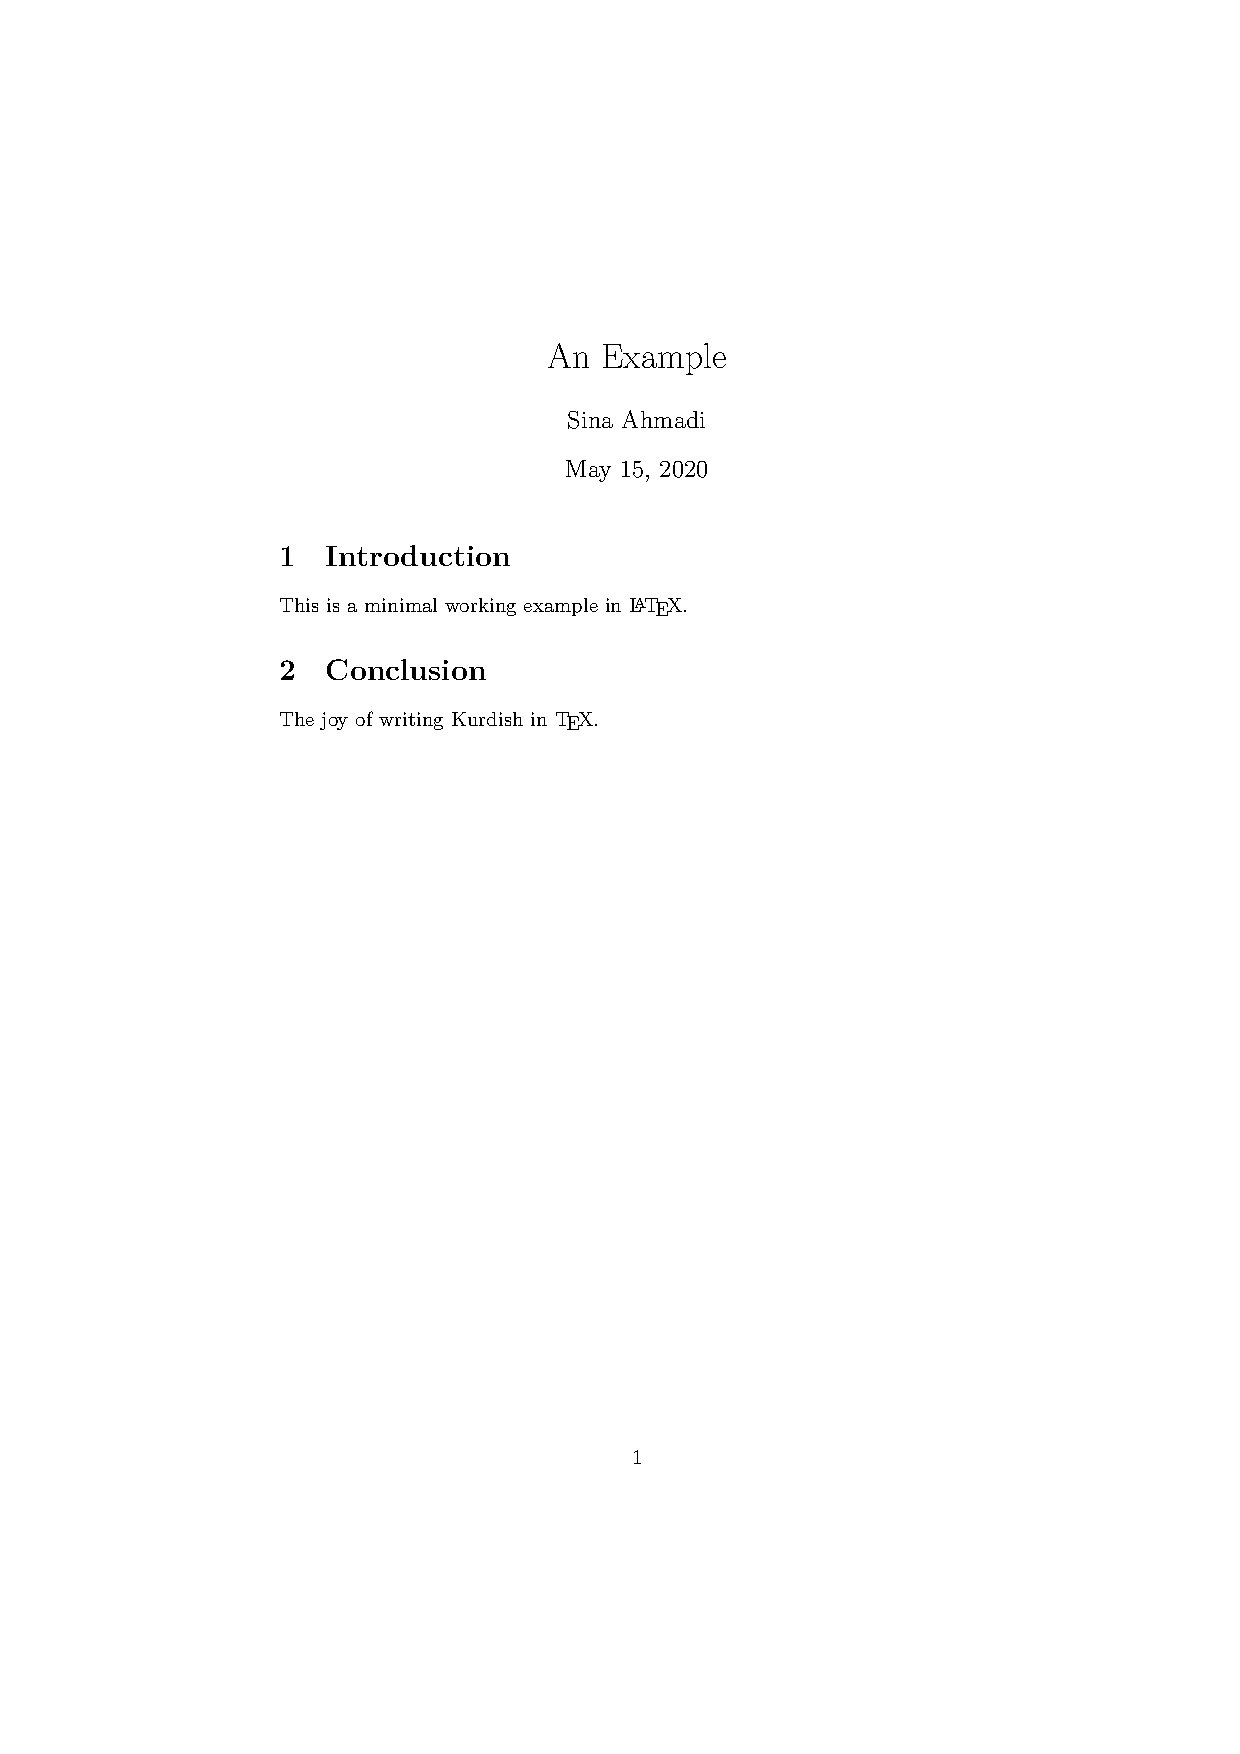
\includegraphics[width=\textwidth]{figure_example.pdf} 
        }
    \end{minipage}
 \caption{Nimûneyek li belgeyek ku bi \LaTeX~hatiye nivîsîn. Li milê çepê, kodê belgeyê ye û li milê rastê jî akamê kampayl kirinê ye}
 \label{fig_mwe}
\end{figure}


Berê, \TeX~tenê çend zimanan  bi tîpên latînî piştgirî dikir û piştra, gelek ziman û nivîsar hatin zêde kirin. \XeLaTeX~li ser \TeX~hate afirandin û li Unicode piştgirî dike. Kurdî gelek zarav û nivîsên wî hene û \XeLaTeX~ji bo wî sîstemek îdeal e, bi taybetî bi bikaranîna \texttt{Polyglossia}\footnote{\url{https://github.com/reutenauer/polyglossia}}. Ji bo afirandina belgeyek bi \XeLaTeX~bi Kurdî, divê belgeya we wiha be:


\begin{lstlisting}
 \documentclass{article}
 \usepackage{polyglossia}

 \setdefaultlanguage[variant=kurmanji,script=latin,numerals=western]{kurdish}

 \begin{document}
 \end{documentu}
\end{lstlisting}

Di rêza yekem de, hûn dibêjin ku belgeya we gotarek e (\texttt{article}). Rêzên 2 heta 4 ji bo bi kar anîna \texttt{Polyglossia} ye û dibêjin ku dixwazin Kurmancî bi rênivîsa Latînî bi kar bînin. Kevala \ref{tab_polyglot_options} sercem vebijarkên \texttt{Polyglossia} ji bo Kurdî nîşan dide.

\begin{table}[h]
\centering
\begin{tabular}{l|l|l|l} 
 \hline
Polyglossia         & variant  & script        & numerals         \\ \hline \hline
\multirow{2}{*}{Kurdish} & \texttt{sorani}   & \texttt{arabic}, \texttt{latin} & \texttt{eastern}, \texttt{western} \\  \cline{2-4} 
                         & \texttt{kurmanji} & \texttt{arabic}, \texttt{latin} & \texttt{eastern}, \texttt{western} \\ \hline
\end{tabular}
\caption{Vebijarkên \texttt{Polyglossia} ji bo afirandina belgeyek bi Kurdî}
\label{tab_polyglot_options}
\end{table}

Bo nimûne, ger hûn dixwazin bi Soranî bi hejmarek tîpên Erebî û rênivîsa Erebî belgeyek çêbikin, hûn mîhengên xwe li rêza 4 wiha diguhezin:

\begin{english}
\begin{lstlisting}
 \setdefaultlanguage[variant=sorani,script=arabic,numerals=eastern]{kurdish}
\end{lstlisting}
\end{english}

Di derbarê salnameyê de, li versîyona niha ji \texttt{Polyglossia}, salnameya zayînî bi tenê heye. Kevala \ref{tab_polyglot_calendar} navên mehan li hemî mîhengan nîşan dide. Bala xwe bidin ku du rewşan hene ji bo nîşan dana tarîxê: \texttt{\textbackslash today} û \texttt{\textbackslash ontoday}. Li rewşê yekem de, tenê navê meha û hejmarên roj û sal tê, bo nimûne, \texttt{30 Gulan 2020}. Lê li rewşê paşîn, \textit{ê} ya Îzafe jî tê, bo nimûne \texttt{30ê Gulanê 2020}. Vê vebijarkê tenê dema karanîna tîpên Latînî peyda dibe.

\begin{table}[h]
\centering
\begin{tabular}{|l|l|l|l|l|} 
\hline
Îngilîsî & Soranî-Erebî & Soranî-Latînî & Kurmancî-Erebî & Kurmancî-Latînî \\\hline\hline
January & {\arabicfont{ دووهەم كانوونی}} & Kanûnî Dûhem  & {\arabicfont{پاشین  چلەیا}} & Çileya Paşîn \\ 
February & {\arabicfont{شوبات}} & Şubat & {\arabicfont{شبات }} & Sibat \\
March & {\arabicfont{ ئازار }} & Azar & {\arabicfont{ ئادار }} & Adar \\
April & {\arabicfont{نیسان }} & Nîsan & {\arabicfont{ نیسان }} & Nîsan \\
May & {\arabicfont{ئایار }} & Ayar & {\arabicfont{ گولان }} & Gulan \\
June & {\arabicfont{حوزەیران }} & Huzeyran & {\arabicfont{ حەزیران }} & Hezîran \\
July & {\arabicfont{ تەممووز }} & Temmûz & {\arabicfont{ تیرمەهـ }} & Tîrmeh \\
August & {\arabicfont{ ئاب }} & Ab & {\arabicfont{ تەباخ }} & Tebax \\
September & {\arabicfont{ئەیلوول }} & Eylûl & {\arabicfont{ ئیلۆن }} & Îlon \\
October & {\arabicfont{  یەكەم تشرینی}} & Tişrînî Yekem & {\arabicfont{  پێشین چریا  }} & Çiriya Pêşîn \\
November & {\arabicfont{  دووهەم تشرینی}} & Tişrînî Dûhem & {\arabicfont{ پاشین چریا }} & Çiriya Paşîn \\
December & {\arabicfont{  یەكەم كانوونی}} & Kanûnî Yekem & {\arabicfont{پێشین چلەیا  }} & Çileya Pêşîn \\ \hline
\end{tabular}
\caption{Navê mehan di salnameya \texttt{Polyglossia}}
\label{tab_polyglot_calendar}
\end{table}

Ji bo zanyarîya zêdetir li ser \texttt{Polyglossia} û zimanê Kurdî, li \cite{Charette2020} û \cite{ahmadi2020TexforKurdish} binihêrin.


\newpage

\section{Çend nimûneyan bi \texttt{Polyglossia}}


\subsection{\XeLaTeX~bo wêje û huner}

\poemtitle*{Yadigarî şîrîn}
\settowidth{\versewidth}{Çawekem! Çawî řeşî to afetî gyanî min e}
\begin{verse}[\versewidth]
çawekem! çawî řeşî to afetî gyanî min e \\
gyanekem! birjangî tîjit nûke řimbî dujmin e \\
\vin şîrî destî şêrî ała ye biro řakşaweket \\
\vin cergî lawêkî hejarî Kurdî wird pê bincine \\ 
çon debê serbest gelî jêrdest ke kiç dabeste bê? \\
bes nebê ew koyletî û ew kiç le jûr dabestine \\
\vin derkî daxistûwe le to babit keçî derkî nîye \\
\vin derke daxistin le to derkî humêd daxistine\\
\end{verse}
\attrib{-- Li dîwana Mamoste Hêminê}



\subsection{\XeLaTeX~bo zanist û bîrkarî}

\begin{center}
\setchemfig{atom sep=2em,bond style={line width=1pt,red,dash pattern=on 2pt off 2pt}}  
\chemname
{\chemfig{H-C(-[2]H)(-[6]H)-C(=[1]O)-[7]H}}
{Êtanal (Ethanal)}
\end{center}


\begin{equation}\label{equation_example}
  x = a_0 + \frac{1}{\displaystyle a_1 
          + \frac{1}{\displaystyle a_2 
          + \frac{1}{\displaystyle a_3 + a_4}}}
\end{equation}


\begin{figure}[h]
\centering
\begin{minipage}[b]{.48\textwidth}
% source of the following: https://www.overleaf.com/learn/latex/CircuiTikz_package
\begin{circuitikz}[american voltages]
\draw
  (0,0) to [short, *-] (6,0)
  to [V, l_=$\mathrm{j}{\omega}_m \underline{\psi}^s_R$] (6,2) 
  to [R, l_=$R_R$] (6,4) 
  to [short, i_=$\underline{i}^s_R$] (5,4) 
  (0,0) to [open, v^>=$\underline{u}^s_s$] (0,4) 
  to [short, *- ,i=$\underline{i}^s_s$] (1,4) 
  to [R, l=$R_s$] (3,4)
  to [L, l=$L_{\sigma}$] (5,4) 
  to [short, i_=$\underline{i}^s_M$] (5,3) 
  to [L, l_=$L_M$] (5,0); 
  \end{circuitikz}
\caption{Serkit bo nimûne}
\label{example_circuit}
\end{minipage}\hfill
\begin{minipage}[b]{.4\textwidth}
  \centering
\begin{tikzpicture}
\begin{axis}[
    title={$x \exp(-x^2-y^2)$}, 
    xlabel=$x$, ylabel=$y$,
	small,
]
\addplot3[
	surf,
	domain=-2:2,
	domain y=-1.3:1.3,
] 
	{exp(-x^2-y^2)*x};
\end{axis}
\end{tikzpicture}
\caption{Fankşinekî matmatîk}
\label{example_function}
\end{minipage}
\end{figure}


\section{Encam}

Di vê gotarê de, me bi kurtahî nîqaş kir çawa \XeLaTeX~bi pakêta \texttt{Polyglossia} ji bo nivîsandina bi Kurdî re bikar tîne. Ji bo zanyarîya zêdetir, biçin \href{https://kurdishxelatex.github.io/}{Koma Bikarînerên \XeLaTeX~ya Kurdî}. Hûn dikarin ji hêla afirandina naverokê jî beşdarî vê komê bibin.


\bibliographystyle{unsrt}
\bibliography{bibliographylatin}

\end{document}
